\documentclass[a4paper,12pt]{article} % добавить leqno в [] для нумерации слева
\usepackage[a4paper,top=1.3cm,bottom=2cm,left=1.5cm,right=1.5cm,marginparwidth=0.75cm]{geometry}
%%% Работа с русским языком
\usepackage{cmap}					% поиск в PDF
\usepackage{mathtext} 				% русские буквы в фомулах
\usepackage[T2A]{fontenc}			% кодировка
\usepackage[utf8]{inputenc}			% кодировка исходного текста
\usepackage[english,russian]{babel}	% локализация и переносы

\usepackage{graphicx}

\usepackage{wrapfig}
\usepackage{tabularx}

\usepackage{hyperref}
\usepackage[rgb]{xcolor}
\hypersetup{
colorlinks=true,urlcolor=blue
}
\usepackage{multirow}
\usepackage{hhline}


%%% Дополнительная работа с математикой
\usepackage{amsmath,amsfonts,amssymb,amsthm,mathtools} % AMS
\usepackage{icomma} % "Умная" запятая: $0,2$ --- число, $0, 2$ --- перечисление

%% Номера формул
\mathtoolsset{showonlyrefs=true} % Показывать номера только у тех формул, на которые есть \eqref{} в тексте.

%% Шрифты
\usepackage{euscript}	 % Шрифт Евклид
\usepackage{mathrsfs} % Красивый матшрифт

%% Свои команды
\DeclareMathOperator{\sgn}{\mathop{sgn}}

%% Перенос знаков в формулах (по Львовскому)
\newcommand*{\hm}[1]{#1\nobreak\discretionary{}
{\hbox{$\mathsurround=0pt #1$}}{}}

\begin{document}
	
	\begin{titlepage}
	\begin{center}
		{\large МОСКОВСКИЙ ФИЗИКО-ТЕХНИЧЕСКИЙ ИНСТИТУТ (НАЦИОНАЛЬНЫЙ ИССЛЕДОВАТЕЛЬСКИЙ УНИВЕРСИТЕТ)}
	\end{center}
	\begin{center}
		{\large Физтех-школа электроники, фотоники и молекулярной физики}
	\end{center}
	
	
	\vspace{4.5cm}
	{\huge
		\begin{center}
			{Лабораторная работа}\\
			Напыление тонких пленок в вакууме
		\end{center}
	}
	\vspace{2cm}
	\begin{flushright}
		{\LARGE Салтыкова Дарья \\
			\vspace{0.5cm}
			Б04-105}
	\end{flushright}
	\vspace{8cm}
	\begin{center}
		Долгопрудный 2022
	\end{center}
\end{titlepage}

\section{Введение}

\noindent
\textbf{Цель работы:} Ознакомление с методами термовакуумного напыления тонких пленок, ионно-плазменными методами (катодным, магнетронными на постоянном токе и высокочастотном), эпитаксиальными методами. Практически получить пленку Al заданной толщины термовакуумным испарением с измерением ее параметров.

\medskip

\noindent
\textbf{Оборудование:} Испаритель (мощный блок питания, вольфрамовая проволока, металлические контакты); вакуумная камера (колпак, прорезиненная подложка(для устранения течей вследствие плохого контакта поверхности с колпаком), насос для предварительной откачки, формвакуумный насос; расходные материалы (проволока из аллюминия, стекло); измерительные приборы (линейка, вакуумметр); прочее (стойка с "лапкой" для удерживания стеклышка, кусачки).

\section{Экспериментальная установка}

\noindent Атомы могут испаряться из жидкой фазы. Конкретная температура испарения подбирается такой, чтобы давление насыщенного пара у поверхности испарителя составило $10^{-2} \text{ мм рт ст}$.

\medskip

\noindent Конструктивно проще всего устроены резистивные испарители, температура которых поддерживается пропусканием электрического тока. Обычно это проволока из тугоплавкого материала, изогнутая в виде шпильки, на нижнем конце которой закрепляется навеска из испаряемого материала. При нагревании навеска плавится, собирается в каплю и удерживается на проволоке силами поверхностного натяжения (рис. 1а). Если испаряемый материал не требует расплавления или не смачивает испаритель, проволоку заменяют лодочкой или плетеной корзинкой (рис. 1б, в, г, ж).

\medskip

\noindent На рисунке представлена схема простейшей вакуумной установки для нанесения пленок. Внутри колпака 9, установленного на плите 1 с герметизирующей прокладкой 2, расположен испаритель 5 с материалом для будущей пленки 4. Подложка 7 нагревается элементом 8 и при достижении заданных режимов испарения открывается заслонкой 6, обычно управляемой электромагнитом.

\medskip

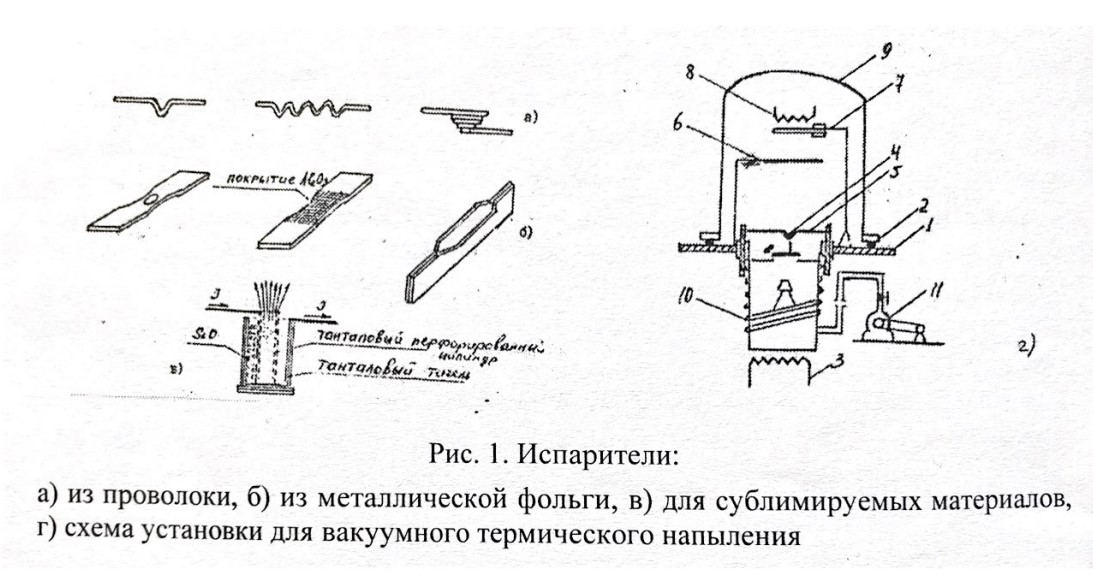
\includegraphics[width=0.6\linewidth]{установка.jpg}
 
 \end{figure}

\medskip
 
\section{Теоретические сведения} 

\noindent При термическом методе испарения различных материалов предусматривается создание вакуума с остаточным давлением не менее $P = 10 \text{мм рт ст}$. Для понимания механизма нанесения тонких пленок необходимо оценить длину свободного пробега атомных частиц остаточных газов, которая должна быть значительно больше расстояния R между испарителем и подложкой. Из кинетической теории газов следует

$$\lambda(\text{см}) = \frac{kT}{4sqrt{2} \pi r^2 p} >> R$$
 
\noindent где T - температура окружающего пространства, P - давление остаточных газов, r - средний радиус атомных частиц (для воздуха $r = 1,87 \cdot 10^{-8} \text{см}$. При комнатной температуре для молекул воздуха получаем

$$ \lambda = \frac{5 \cdot 10^{-2}}{p \text{мм рт ст}.}$$

\noindent То есть в вакууме P = 10 мм рт ст длина свободного пробега составляет ~50 см, что значительно больше расстояния испаритель-подложка (10 см).

\medskip

\noindent Пользуясь сферической геометрией распределения испаряемых атомов из точечного источника можно вывести формулу зависимости толщины тонкой пленки в зависимости от массы испаряемого вещества и расстояние $R_0$ от источника до подложки.

\medskip

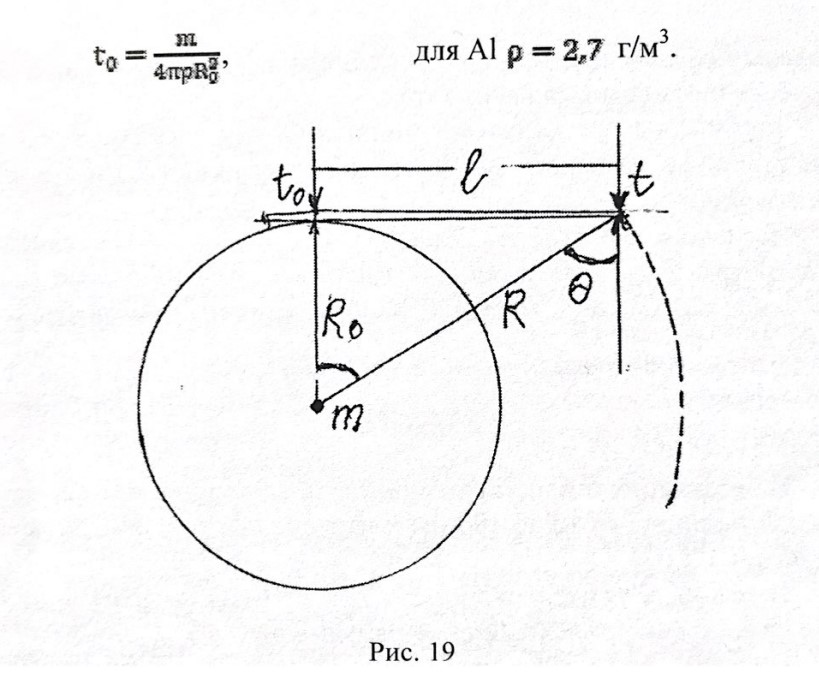
\includegraphics[width=0.6\linewidth]{круг.jpg}
 \end{figure}
 
 \medskip

\section{Обработка результатов}

\noindent Рассчитаем $t_0$ и оценим погрешность. Используя метод частных производных: 

$$\Delta t_{0} = |\operatorname{grad}t_{0} \cdot \Delta_{t_{0}}|{2}=\sqrt{\frac{\left|{\frac{\Delta{m}}{R^{2} \rho}}\right|^{2}}{16 \pi^{2}} + \frac{\left|{\frac{\Delta_{R} m}{R^{3} \rho}}\right|^{2}}{4 \pi^{2}} + \frac{\left|{\frac{\Delta_{\rho} m}{R^{2} \rho^{2}}}\right|^{2}}{16 \pi^{2}}} $$ 

\noindent Подставив данные эксперимента получаем:

$$ t_0 = 13 \pm 1 \text{ нм}.$$

\noindent Теперь оценим толщину, используя данные спектрометра:


\medskip
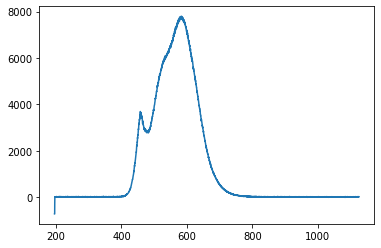
\includegraphics[width=0.7\linewidth]{свет.png}
 	\caption
 	
 {Спектр освещения лампочки}
 \end{figure}
 
 \medskip
 
 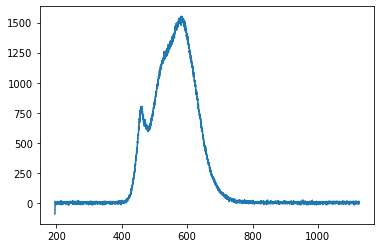
\includegraphics[width=0.7\linewidth]{спектр1.png}
 	\caption
 	
 	\medskip
 	{Спектр при просвечивании лампочки через стекло с нанесённым алюминиевым покрытием}
 \end{figure}

\medskip

\noindent Проинтегрируем данные функции, чтобы получить полный поток:

$$\int\limits_{200}^{1000} \Phi(\lambda)d\lambda$$

\noindent Коэффициент пропускания определяется как отношения потока, пропущенного через материал, к потоку, падающему на материал:

$$ T = \frac{\Phi}{\Phi_0}$$

\noindent В результате вычисления T различными способами получаем T = 22. Согласно графику,

\medskip

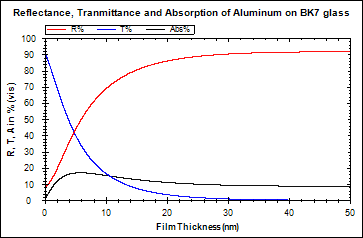
\includegraphics[width=0.7\linewidth]{табл.png}
 
 \end{figure}
 
 \medskip


\noindent толщина плёнки алюминия при таком коэффициенте пропускания есть 10 нм.

\noindent Согласно расчётам, сделанным ранее, получили, что максимальная толщина плёнки $t_0 = 13 \pm 1$ нм. Воспользуемся формулой распределения толщины, и получим, что минимальная толщина есть $t_{min} = 10,5 \pm 0,8 \text{ нм}$.

\section{Вывод}

\noindent В ходе работы была получена алюминиевая пленка с минимальной толщиной $t_{min} = 10,5 \pm 0,8 \text{ нм}$.
\medskip

\end{document}